\problemname{Golvyta}
\noindent
Du ska snart sälja ditt hus, men först måste du räkna ut hur stor golvytan är. Det 
kanske låter lätt, men du har ett oanvänt förråd som du glömt nyckeln till,
och du har ingen aning om hur stort det är. Det enda som finns i förrådet är en robotdammsugare.
Om du sätter igång dammsugaren och kollar vart den hamnar, så kanske du kan räkna ut hur 
stort förrådet är?

Förrådet består av ett $N \times M$ rutnät, där $N$ och $M$ är okända positiva heltal. Raderna är numrerade från $0$ till $N-1$ uppifrån 
och ned, och kolumnerna är numrerade från $0$ till $M-1$ från vänster till höger. Roboten 
har en lista med instruktioner $s$. Denna beskrivs av en sträng som består av tecknen \verb|<|, \verb|>|, \verb|^|, 
och \verb|v|. När roboten sätts igång läser den dessa instruktioner,
och för var och en åker den ett steg i motsvarande riktning. Om roboten försöker åka utanför rutnätet så åker 
den in i väggen och ingenting händer. Roboten startar i övre vänstra hörnet, alltså på 
rad $0$ och kolumn $0$.

Du får givet strängen $s$ och vilken rad och kolumn roboten hamnade på efter att den följt instruktionerna.
Räkna ut det minsta möjliga värdet på $N\cdot M$ som stämmer överens med denna information.


\section*{Indata}
Den första raden innehåller ett heltal $K$ ($1 \leq K \leq 3 \cdot 10^5$), längden på strängen $s$.

Den andra raden innehåller strängen $s$.

Den tredje raden innehåller två heltal $r$ och $c$ ($0 \leq r,c < 3 \cdot 10^5$), där
$r$ är vilken rad roboten hamnade på och $c$ är vilken kolumn den hamnade på.

\section*{Utdata}
Skriv ut ett heltal, det minsta möjliga värdet på $N \cdot M$. Om det inte finns något val av 
$N$ och $M$ som stämmer överens med informationen i testdatan, så ska du istället skriva 
ut $-1$. 

\section*{Poängsättning}
Din lösning kommer att testas på en mängd testfallsgrupper.
För att få poäng för en grupp så måste du klara alla testfall i gruppen.

\noindent
\begin{tabular}{| l | l | p{12cm} |}
  \hline
  \textbf{Grupp} & \textbf{Poäng} & \textbf{Gränser} \\ \hline
  $1$    & $15$       & Roboten går bara nedåt och åt höger. \\ \hline
  $2$    & $30$       & $K \leq 100$ \\ \hline
  $3$    & $20$       & $K \leq 5000$ \\ \hline
  $4$    & $35$       & Inga ytterligare begränsningar. \\ \hline
\end{tabular}

\section*{Förklaring av exempelfall}
\begin{centering}
  \begin{figure}[h]
      \centering
      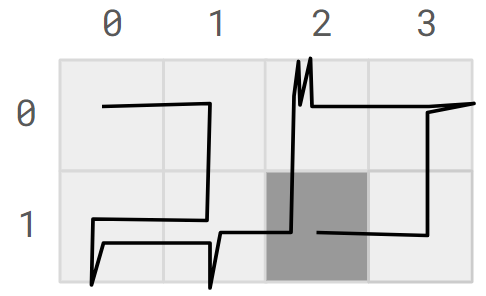
\includegraphics[width=0.4\textwidth]{golvyta.PNG}
      \caption{Bilden visar det minsta möjliga rutnätet i sample 1. Roboten färdas enligt den svarta kurvan. Den mörka rutan är robotens slutgiltiga position.}
  \end{figure}
\end{centering}
